\documentclass[11pt]{article}

\usepackage[top=0.5in, bottom=0.5in, left=0.5in, right=0.5in]{geometry}
\usepackage{authblk}
\usepackage{hyperref}
\usepackage[utf8]{inputenc}
\usepackage{amsmath}
\usepackage{amsfonts}
\usepackage{amssymb}
\usepackage{siunitx}
\usepackage{graphicx}
\usepackage{subcaption}
\usepackage{float}
\usepackage[nottoc,numbib]{tocbibind}
\usepackage{biblatex}

% For Diagrams
\usepackage{tikz}

\bibliography{references.bib}

\newcommand{\email}[1]{\texttt{\href{mailto:#1}{#1}}}

\title{A Deep Learning Approach to Finding the Initial Conditions of the Universe}
% \author{\small Aarti Singh\footnote{Associate Professor, Machine Learning Department, Carnegie Mellon University, \email{aarti@cs.cmu.edu}}, Albert Liang\footnote{Graduate student, Machine Learning Department, Carnegie Mellon University, \email{ajliang@cs.cmu.edu}}, Vaibhav Jindal\footnote{Graduate Student, Machine Learning Department, Carnegie Mellon University, \email{vjindal@cs.cmu.edu}}}

\makeatletter
\let\inserttitle\@title
% \let\insertauthor\@author
\makeatother

\begin{document}

\begin{center}
  \LARGE{\inserttitle}

  % \Large{\insertauthor}
\end{center}

\section{Abstract}

We introduce a novel neural-network based method to predict the linear inputs of an N-body simulation given its non-linear displacement at redshift zero. 
We train a V-Net based convolutional neural network, which outputs the linear displacement of an N-body system, given the current time non-linear displacement and the cosmolgical parameters of the system.
Since the mapping between the non-linear displacements to the linear displacements is one-to-many, training a neural network for such predictions is essentially ill-defined because of the one-to-one nature of neural network mappings. 
However, in this work, we demonstrate that neural networks can accurately recover the initial displacement field on large scales despite the ill-defined nature of the problem.
This is the first work that tries to use a neural network to predict the initial conditions of the universe given the current time conditions.
The results of our method motivate that neural network based models can act as good approximators of the initial linear states and their predictions can serve as good starting points for sampling-based methods to infer the initial states of the universe.

\section{Introduction}

The evolution of our universe can be uniquely determined by its initial conditions and the laws of physics governing its dynamics. To understand the evolution of  universe, astrophysicists use a large number of simulations to extract meaningful information. These simulations try to predict the non-linear structure of a system of N-body particles given the initial conditions of these particles. These forward simulations, however, are computationally expensive and require a large amount of time.

In recent years, deep-learning has shown to be extremely helpful in accelerating the forward modelling process \cite{he_li_feng_ho_ravanbakhsh_chen_póczos_2019}. These deep-learning models learn from pairs of inputs and outputs from actual physical N-body simulations and act as fast and accurate approximators for these simulators. These deep-learning surrogates speed up the forward modelling process by orders of magnitude. Since neural networks are theoretically proven to be universal function approximators, the forward modelling of N-body simulations fits perfectly into the regime of neural networks.
\begin{figure}[h!]
    \centering
    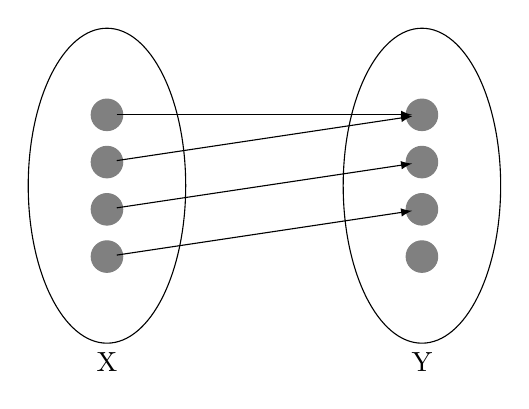
\begin{tikzpicture}
  % Set X oval
  \draw (-2,0) ellipse (1 and 2);
  \draw (-2,-2) node[below] {X};
  % Set X elements
  \draw[gray, fill=gray] (-2,0.9) circle (0.2) node (x1) {};
  \draw[gray, fill=gray] (-2,0.3) circle (0.2) node (x2) {};
  \draw[gray, fill=gray] (-2,-0.3) circle (0.2) node (x3) {};
  \draw[gray, fill=gray] (-2,-0.9) circle (0.2) node (x4) {};
  
  % Set Y oval
  \draw (2,0) ellipse (1 and 2);
  \draw (2,-2) node[below] {Y};
  % Set Y elements
  \draw[gray, fill=gray] (2,0.9) circle (0.2) node (y1) {};
  \draw[gray, fill=gray] (2,0.3) circle (0.2) node (y2) {};
  \draw[gray, fill=gray] (2,-0.3) circle (0.2) node (y3) {};
  \draw[gray, fill=gray] (2,-0.9) circle (0.2) node (y4) {};
  
  % Arrows
  \draw[-latex] (x1) -- (y1);
  \draw[-latex] (x2) -- (y1);
  \draw[-latex] (x3) -- (y2);
  \draw[-latex] (x4) -- (y3);
\end{tikzpicture}
    \caption{Example of a many-to-one function between two sets X and Y. For our purpose, X corresponds to the set of all possible initial conditions of an N-body simulation and Y corresponds to the set of final conditions.}
    \label{manytoone}
\end{figure}

The problem of inferring the initial state of the universe, or an N-body simulation, however poses a completely different challenge because multiple different initial states could lead to the same final state, i.e., it is a many-to-one function; Figure \ref{manytoone}. Thus, the mapping from final states to the initial states is not a function, but rather a one-to-many relation. Therefore, there is no direct way of determining the initial conditions and we must resort to progressive sampling based methods to infer possible initial states. Although counter-intuitive to the nature of the problem, we try to attack this problem by learning a deterministic neural network to output the initial states for a given output state. We show that despite the one-to-many nature of the mapping, a simple neural network, when trained to predict the initial state for a given output state, can do an excellent job of predicting the initial states at large scales. Our results empirically motivate the use of neural networks as approximate inverse-mapping black boxes that could generate reliable initial states for a given output state, which could then be used to speed-up the more fine-grained sampling-based inverse modelling methods.

\section{Methods}

We train a CNN based neural network to predict the initial state of an N-body system of particles evolving under gravity on an expanding cosmological background, given the final state. Our CNN takes the nonlinear displacement field at redshift $z=0$ and the value of $\mathbf{\Omega}_m$ as the input, and predicts the linear displacement field, i.e., the Zel'dovich approximation (ZA) at redshift $z=0$.

\begin{figure*}[t!]
\begin{center}
\centerline{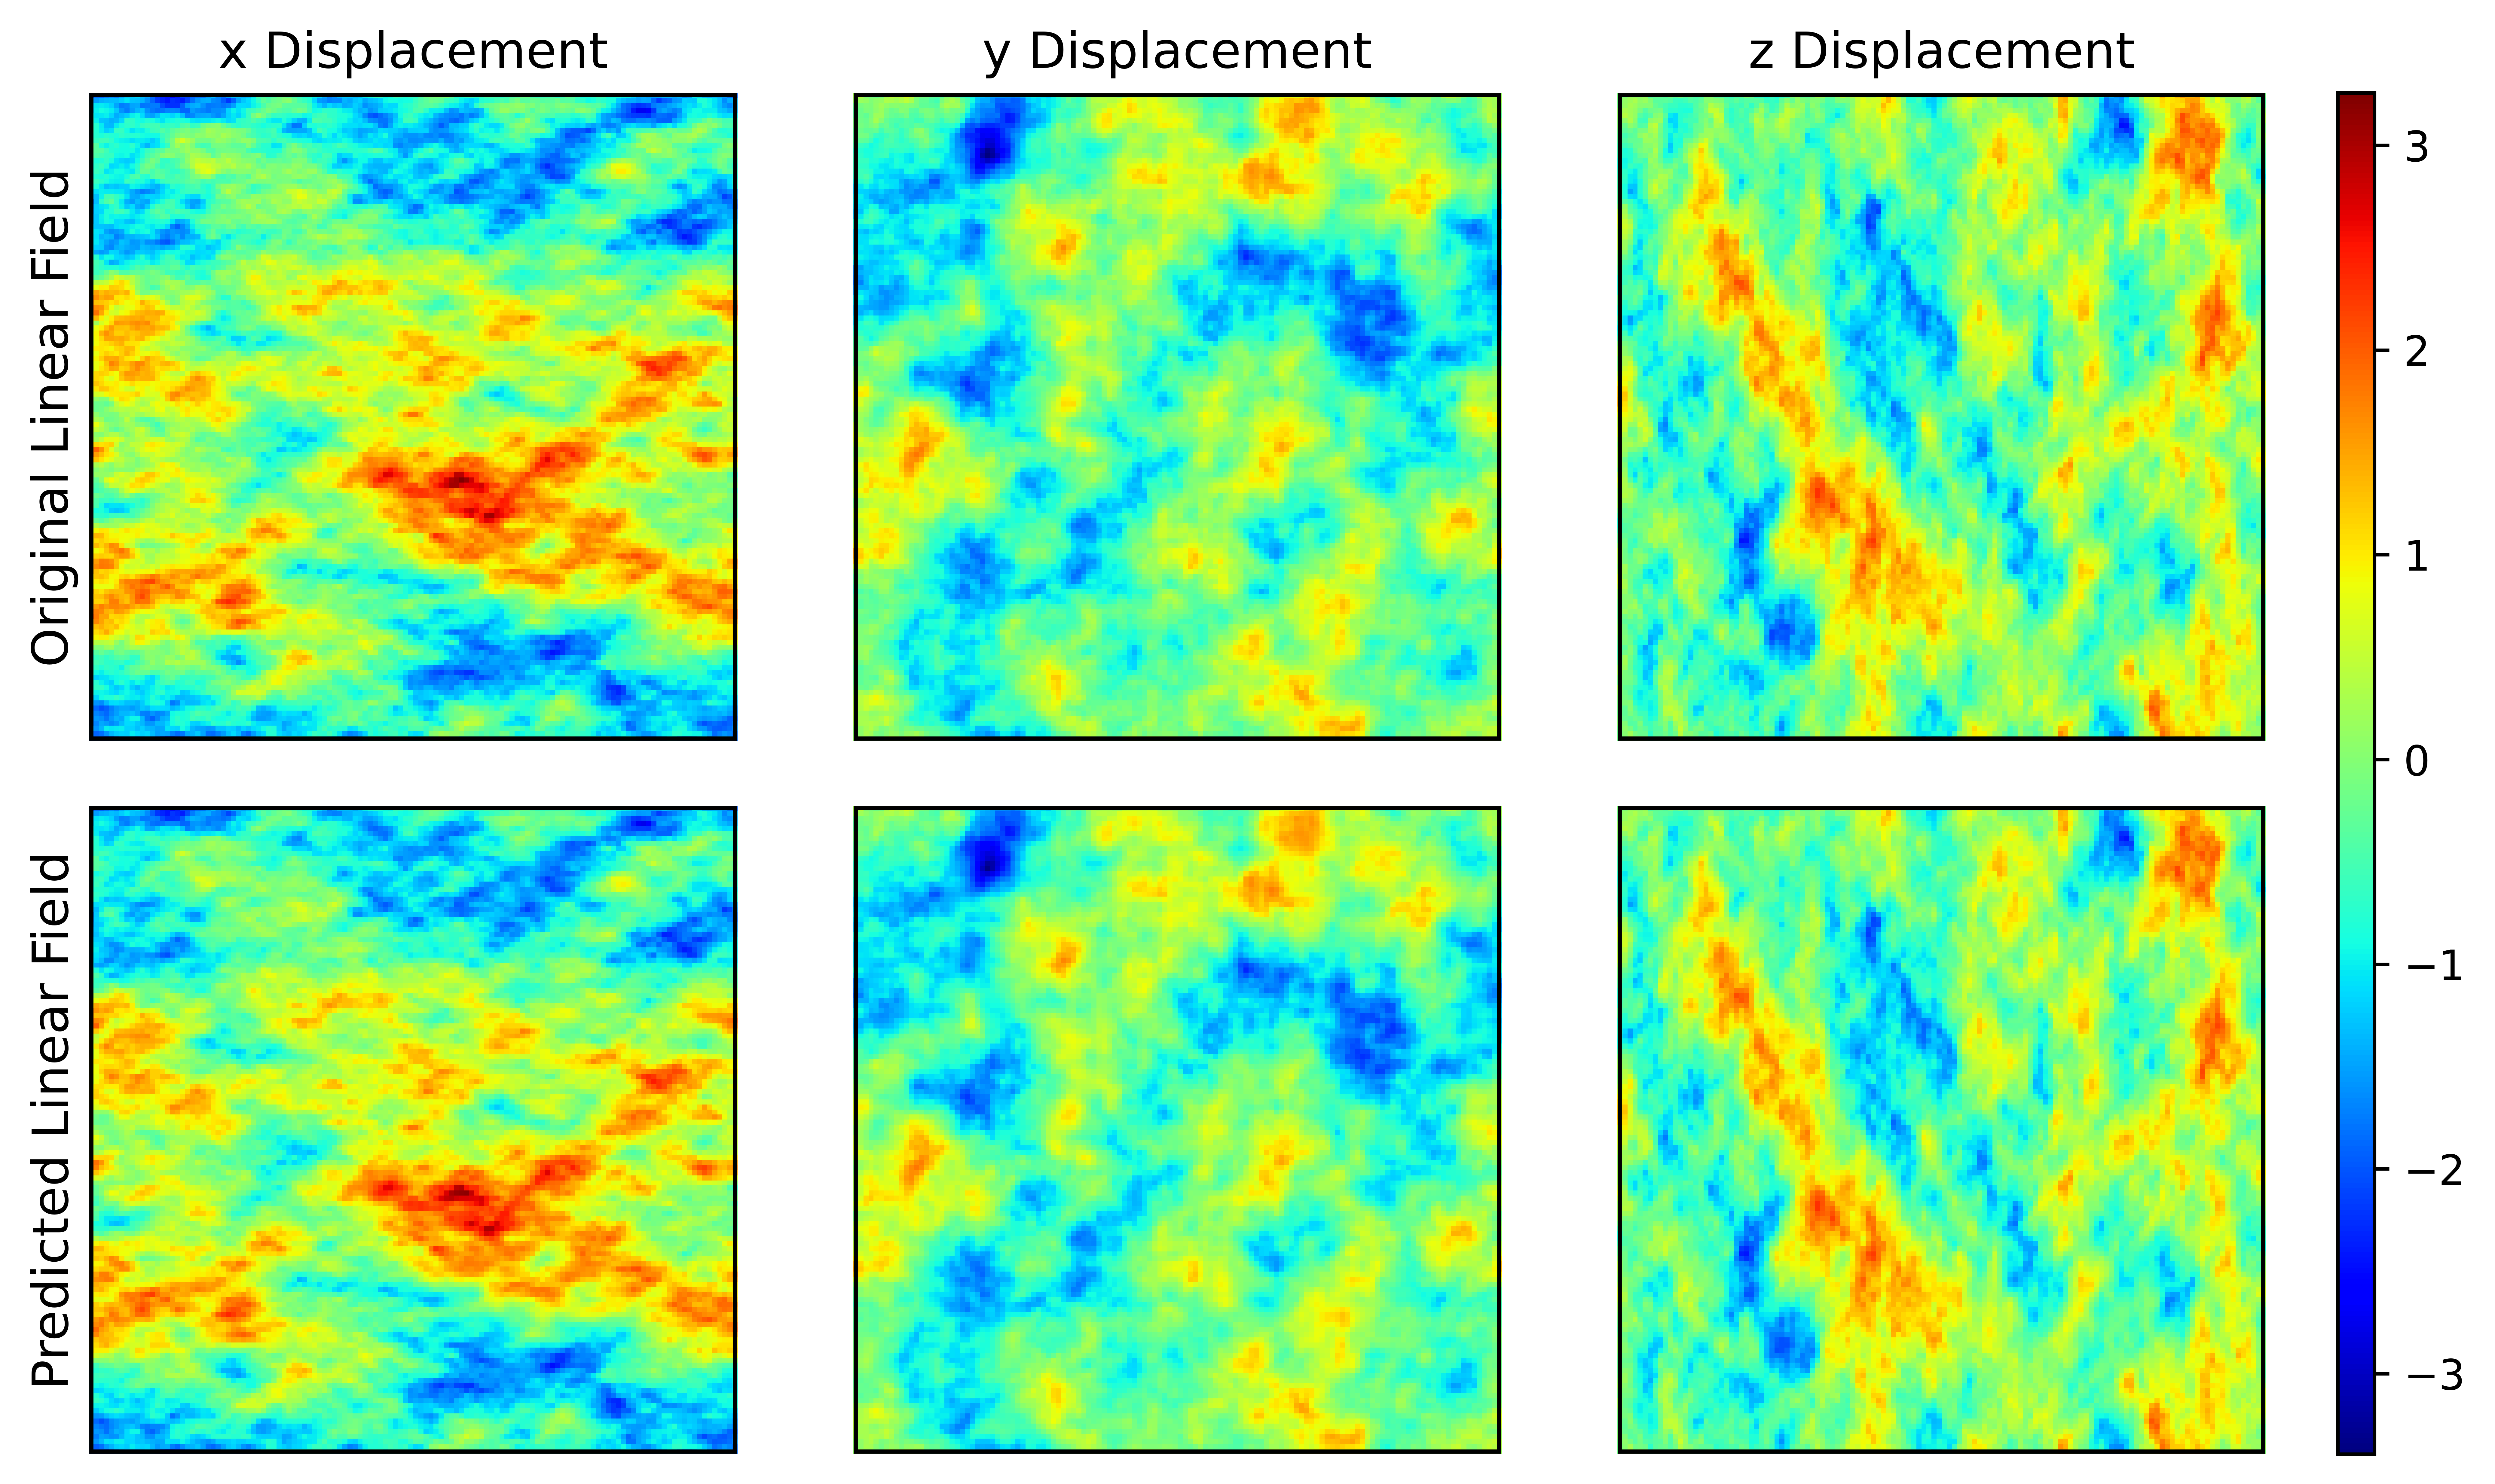
\includegraphics[width=0.8\textwidth]{images/slices.png}}
\caption{Qualitative comparison between a $128 \times 128$ slice of particles from the original linear field (target) and the corresponding linear field predicted by our inverse model (prediction). The plots show the $x,y, \text{and } z$ displacements for the two fields.}
\label{slices}
\end{center}
\end{figure*}

Consider an N-body system with particles distributed on a uniform grid with positions $\mathbf{q}$. Let $\mathbf{\Psi}_{ZA}(\mathbf{q})$ be their linear ZA approximation at redshift $z=0$. Thus, the final positions of the particles when they evolve linearly according to the Zel'dovich approximation is
$$\mathbf{x}_{lin}(\mathbf{q}) = \mathbf{q} + \mathbf{\Psi}_{ZA}(\mathbf{q}).$$
Let the final non-linear displacement of the particle initially at grid site $\mathbf{q}$ be $\mathbf{\Psi}_{NL}(\mathbf{q})$. Thus, the final positions of the particles at redshift $z=0$ under non-linear evolution is 
$$\mathbf{x}_{non-lin}(\mathbf{q}) = \mathbf{q} + \mathbf{\Psi}_{NL}(\mathbf{q}).$$
We train our CNN to output the linear displacement field $\mathbf{\Psi}_{ZA}(\mathbf{q})$ for a given non-linear displacement field $\mathbf{\Psi}_{NL}(\mathbf{q})$, and a given value of the $\mathbf{\Omega}_m$.
We directly use the CNN architecture used in \cite{https://doi.org/10.48550/arxiv.2206.04594} and train it using xxx pairs of non-linear and linear displacement fields from the Quijote simulation suite \cite{villaescusa}. In terms of the training procedure, our method is almost exactly similar to \cite{https://doi.org/10.48550/arxiv.2206.04594}, with the only difference being that we reversed the inputs and outputs of the neural network. We now input the non-linear field to our CNN and ask it to predict the linear field. This is exactly opposite to what was being done by \cite{https://doi.org/10.48550/arxiv.2206.04594}.

For our experiments, we use simulations of $128^3$ particles in a square box with a side-length of $250 h^{-1}$Mpc. The particles are distributed uniformly across this grid with a mean separation of $\sim1.95 h^{-1}$Mpc between two adjacent particles of the grid.

\section{Initial Results}

\textit{How would you carry out the analysis? What kind of analysis (or analyses) do you plan to use? There should be reasonable justification of candidate methods. You may learn methods you plan to use later in the semester. The final project report should focus on this section.}

\section{Resource Request}

Calculate size of 2000 Quijote simulation:

Linear input size: 1.61GB

Nonlinear output size: 1.61GB

Total size = $2000 \cdot (1.61 + 1.61) = 6,440$GB

\pagebreak

\printbibliography

\end{document}